% Options for packages loaded elsewhere
% Options for packages loaded elsewhere
\PassOptionsToPackage{unicode}{hyperref}
\PassOptionsToPackage{hyphens}{url}
\PassOptionsToPackage{dvipsnames,svgnames,x11names}{xcolor}
%
\documentclass[
  10pt,
  ignorenonframetext,
  aspectratio=1610,
]{beamer}
\newif\ifbibliography
\usepackage{pgfpages}
\setbeamertemplate{caption}[numbered]
\setbeamertemplate{caption label separator}{: }
\setbeamercolor{caption name}{fg=normal text.fg}
\beamertemplatenavigationsymbolsempty
% remove section numbering
\setbeamertemplate{part page}{
  \centering
  \begin{beamercolorbox}[sep=16pt,center]{part title}
    \usebeamerfont{part title}\insertpart\par
  \end{beamercolorbox}
}
\setbeamertemplate{section page}{
  \centering
  \begin{beamercolorbox}[sep=12pt,center]{section title}
    \usebeamerfont{section title}\insertsection\par
  \end{beamercolorbox}
}
\setbeamertemplate{subsection page}{
  \centering
  \begin{beamercolorbox}[sep=8pt,center]{subsection title}
    \usebeamerfont{subsection title}\insertsubsection\par
  \end{beamercolorbox}
}
% Prevent slide breaks in the middle of a paragraph
\widowpenalties 1 10000
\raggedbottom
\usepackage{iftex}
\ifPDFTeX
  \usepackage[T1]{fontenc}
  \usepackage[utf8]{inputenc}
  \usepackage{textcomp} % provide euro and other symbols
\else % if luatex or xetex
  \usepackage{unicode-math} % this also loads fontspec
  \defaultfontfeatures{Scale=MatchLowercase}
  \defaultfontfeatures[\rmfamily]{Ligatures=TeX,Scale=1}
\fi
\usepackage{lmodern}

\ifPDFTeX\else
  % xetex/luatex font selection
\fi
% Use upquote if available, for straight quotes in verbatim environments
\IfFileExists{upquote.sty}{\usepackage{upquote}}{}
\IfFileExists{microtype.sty}{% use microtype if available
  \usepackage[]{microtype}
  \UseMicrotypeSet[protrusion]{basicmath} % disable protrusion for tt fonts
}{}
\makeatletter
\@ifundefined{KOMAClassName}{% if non-KOMA class
  \IfFileExists{parskip.sty}{%
    \usepackage{parskip}
  }{% else
    \setlength{\parindent}{0pt}
    \setlength{\parskip}{6pt plus 2pt minus 1pt}}
}{% if KOMA class
  \KOMAoptions{parskip=half}}
\makeatother


\usepackage{longtable,booktabs,array}
\newcounter{none} % for unnumbered tables
\usepackage{calc} % for calculating minipage widths
\usepackage{caption}
% Make caption package work with longtable
\makeatletter
\def\fnum@table{\tablename~\thetable}
\makeatother
\usepackage{graphicx}
\makeatletter
\newsavebox\pandoc@box
\newcommand*\pandocbounded[1]{% scales image to fit in text height/width
  \sbox\pandoc@box{#1}%
  \Gscale@div\@tempa{\textheight}{\dimexpr\ht\pandoc@box+\dp\pandoc@box\relax}%
  \Gscale@div\@tempb{\linewidth}{\wd\pandoc@box}%
  \ifdim\@tempb\p@<\@tempa\p@\let\@tempa\@tempb\fi% select the smaller of both
  \ifdim\@tempa\p@<\p@\scalebox{\@tempa}{\usebox\pandoc@box}%
  \else\usebox{\pandoc@box}%
  \fi%
}
% Set default figure placement to htbp
\def\fps@figure{htbp}
\makeatother





\setlength{\emergencystretch}{3em} % prevent overfull lines

\providecommand{\tightlist}{%
  \setlength{\itemsep}{0pt}\setlength{\parskip}{0pt}}



 


%%%============================================================
%%%  UCL Beamer theme
%%%  Companion to the UCL 2026 revealjs Quarto extension
%%%  Requires: xelatex (or lualatex), fontspec, tikz, tcolorbox,
%%%            soul, xcolor, fontawesome5, unicode-math
%%%============================================================

\usepackage{fontspec}
\usepackage{tikz}
\usepackage[most]{tcolorbox}
\usepackage{soul}
\usepackage{xcolor}
\usepackage{fontawesome5}
\usetikzlibrary{calc, positioning}

% Per-frame boolean: true = skip logo on this frame. Set by the lua
% filter when a slide heading has {.no-logo}; reset by the footline
% template after each frame, so the effect is local to one slide.
\newif\ifuclNoLogo

%%%------------------------------------------------------------
%%%  MathJax / Unicode-Math compatibility
%%%------------------------------------------------------------
\usepackage{unicode-math}

% Cleanly override math bold formatting macros for LuaLaTeX
\protected\def\bm#1{\symbf{#1}}
\protected\def\boldsymbol#1{\symbf{#1}}

% Restore the familiar Computer Modern calligraphic \mathcal.
% unicode-math points \mathcal at the math font's script slot, which
% for Latin Modern Math looks quite different from the classical LaTeX
% calligraphic that most maths papers use. This override sends
% \mathcal back to CM Math Symbols (OMS/cmsy) — same glyphs as
% pdflatex + amssymb, so \mathcal{S}, \mathcal{D} etc. look expected.
\DeclareMathAlphabet{\mathcal}{OMS}{cmsy}{m}{n}

%%%------------------------------------------------------------
%%%  MathJax compatibility
%%%------------------------------------------------------------
% MathJax's \class{name}{content} attaches an HTML class for CSS
% styling. In your source it's used as \class{colour}{expression}.
% Define it here as a colour wrapper so beamer renders the same
% intent — content typeset in the named colour.
\def\class#1#2{{\color{#1}#2}}

%%%------------------------------------------------------------
%%%  Path constants (adjust here if your extension layout differs)
%%%------------------------------------------------------------
% Resolved relative to the project root (where the .qmd lives).
% If you compile from a subfolder, use absolute paths instead.
\newcommand{\UCLfontpath}{css/fonts/}
\newcommand{\UCLimgpath}{images/}

%%%------------------------------------------------------------
%%%  Fonts
%%%------------------------------------------------------------
% UCLSans has Regular + Bold + SemiBold TTFs. There is no italic,
% so we synthesise one with AutoFakeSlant.
\setmainfont{UCLSans}[
  Path             = \UCLfontpath,
  Extension        = .ttf,
  UprightFont      = *-Regular,
  BoldFont         = *-Bold,
  FontFace         = {sb}{n}{*-SemiBold},
  AutoFakeSlant    = 0.18,
]
\setsansfont{UCLSans}[
  Path             = \UCLfontpath,
  Extension        = .ttf,
  UprightFont      = *-Regular,
  BoldFont         = *-Bold,
  FontFace         = {sb}{n}{*-SemiBold},
  AutoFakeSlant    = 0.18,
]
% Monospace: use Ubuntu Mono if the system has it, else fall back
% silently to the LaTeX default (Latin Modern Mono).
\IfFontExistsTF{Ubuntu Mono}{%
  \setmonofont{Ubuntu Mono}[Scale=0.90]%
}{}

%%%------------------------------------------------------------
%%%  Colours (UCL palette)
%%%------------------------------------------------------------
\definecolor{uclbrightpurple}{HTML}{993BFF}
\definecolor{ucldarkpurple}{HTML}{361A54}
\definecolor{uclnavy}{HTML}{002248}   % headings on light bg
\definecolor{uclblue}{HTML}{002855}   % 'uclblue' class
\definecolor{uclbg}{HTML}{FAFAFA}     % body background / light text
\definecolor{ucltext}{HTML}{00142B}   % body text
\definecolor{uclgold}{HTML}{C6AA51}   % links
\definecolor{ucldarkgold}{HTML}{AC8300} % list markers
\definecolor{uclhighlight}{HTML}{715600}
\definecolor{ucllink}{HTML}{95A6B8}
\definecolor{uclfootertext}{HTML}{CCD1D5}

% Named colour classes used inline as [text]{.classname}
% Names match the CSS class names 1:1 so the lua filter can map them.
\definecolor{myred}{HTML}{E62B4F}
\definecolor{myblue}{HTML}{24568C}
\definecolor{orange}{HTML}{FF8811}
\definecolor{olive}{HTML}{334F17}
\definecolor{ubuntublue}{HTML}{035AA6}
\definecolor{spanish-red}{HTML}{C60B1E}
\definecolor{spanish-yellow}{HTML}{FFC400}
\definecolor{italian-green}{HTML}{009246}
\definecolor{italian-red}{HTML}{CE2B37}
\definecolor{blue90red60}{HTML}{7E5DC9}
\definecolor{blue60red90}{HTML}{9350C7}
\definecolor{lightgray}{HTML}{EDEDED}
\definecolor{navbargrey}{HTML}{D5D5D5}
\definecolor{beamer-yellow}{HTML}{FCD000}
\definecolor{samp-blue}{HTML}{1B5497}
\definecolor{samp-red}{HTML}{C21718}
\definecolor{magenta}{HTML}{FF00FF}

%%%------------------------------------------------------------
%%%  PDF viewer hints
%%%------------------------------------------------------------
% Ask the viewer to fit the whole page and open in fullscreen.
% Not all viewers honour these; evince respects pdfstartview but
% F5 (presentation mode) is more reliable than F11 for talks.
\hypersetup{
  pdfstartview  = Fit,
%  pdfpagemode   = FullScreen,
}


%%%------------------------------------------------------------
%%%  Beamer colour scheme
%%%------------------------------------------------------------
\setbeamercolor{normal text}{fg=ucltext, bg=uclbg}
\setbeamercolor{background canvas}{bg=uclbg}
\setbeamercolor{structure}{fg=ucldarkpurple}
\setbeamercolor{alerted text}{fg=uclbrightpurple}
\setbeamercolor{example text}{fg=ucldarkgold}

\setbeamercolor{frametitle}{fg=ucldarkpurple, bg=uclbg}
\setbeamercolor{title}{fg=uclbg}
\setbeamercolor{subtitle}{fg=uclbg}
\setbeamercolor{author}{fg=uclbg}
\setbeamercolor{date}{fg=uclbg}
\setbeamercolor{institute}{fg=uclbg}

\setbeamercolor{itemize item}{fg=ucldarkgold}
\setbeamercolor{itemize subitem}{fg=ucldarkgold}
\setbeamercolor{itemize subsubitem}{fg=ucldarkgold}
\setbeamercolor{enumerate item}{fg=ucldarkgold}
\setbeamercolor{enumerate subitem}{fg=ucldarkgold}

\setbeamercolor{block title}{fg=uclbg, bg=ucldarkpurple}
\setbeamercolor{block body}{fg=ucltext, bg=uclbg!92!ucldarkpurple}

%%%------------------------------------------------------------
%%%  Beamer fonts (Perfect Widescreen Balance)
%%%------------------------------------------------------------
\setbeamerfont{subtitle}{family=\sffamily, size=\normalsize}
\setbeamerfont{author}{family=\sffamily, series=\bfseries, size=\small}
\setbeamerfont{date}{family=\sffamily, size=\footnotesize}
\setbeamerfont{institute}{family=\sffamily, size=\footnotesize}
\setbeamerfont{footline}{family=\sffamily, size=\scriptsize}

% Frame title = 1.5× body (matches PowerPoint 36pt title / 24pt body).
% We capture the documentclass base font size in \uclbasesize at
% BeginDocument, then compute the title size proportionally. This means
% changing 'fontsize:' in YAML scales the frame title with everything else.
\newlength{\uclbasesize}
\makeatletter
\AtBeginDocument{\uclbasesize=\f@size pt}
\makeatother
\setbeamerfont{frametitle}{family=\sffamily, series=\bfseries,
  size=\fontsize{\dimexpr1.5\uclbasesize\relax}{\dimexpr1.8\uclbasesize\relax}\selectfont}
\setbeamertemplate{frametitle}{%
  \nointerlineskip
  \vspace{0.6ex}
  \begin{beamercolorbox}[wd=\paperwidth, ht=3.5ex, dp=1.2ex,
                         leftskip=0.05\paperwidth]{frametitle}%
    \usebeamerfont{frametitle}\usebeamercolor[fg]{frametitle}%
    \insertframetitle%
  \end{beamercolorbox}%
}

% Body text: no hardcoded size — respects documentclass fontsize option.
% Line spacing is left at beamer's default (tight but readable); if you want
% more airy body text, add \linespread{1.05}\selectfont here.


%%%------------------------------------------------------------
%%%  Inner theme (bullets, blocks)
%%%------------------------------------------------------------
\setbeamertemplate{navigation symbols}{}
\useinnertheme{default}

% Bullet markers: filled square in ucldarkgold to match CSS ::marker
\setbeamertemplate{itemize item}{%
  \raisebox{0.15ex}{\color{ucldarkgold}\rule{0.55ex}{0.55ex}}}
\setbeamertemplate{itemize subitem}{%
  \raisebox{0.15ex}{\color{ucldarkgold}\rule{0.45ex}{0.45ex}}}
\setbeamertemplate{itemize subsubitem}{%
  \raisebox{0.15ex}{\color{ucldarkgold}\rule{0.35ex}{0.35ex}}}

% Enumerate: bold gold numbers
\setbeamertemplate{enumerate item}{\color{ucldarkgold}\bfseries\insertenumlabel.}

% Blocks: rounded, coloured header bar
\setbeamertemplate{block begin}{%
  \setbeamercolor{block title}{fg=uclbg, bg=ucldarkpurple}%
  \begin{beamercolorbox}[colsep*=.75ex, sep=0.4ex, rounded=true]{block title}%
    \usebeamerfont*{block title}\insertblocktitle
  \end{beamercolorbox}%
  \nointerlineskip
  \begin{beamercolorbox}[colsep*=.75ex, sep=0.6ex, vmode, rounded=true]{block body}%
}
\setbeamertemplate{block end}{\end{beamercolorbox}\vspace*{0.5ex}}

% Blockquotes
\newenvironment{uclquote}{%
  \begin{tcolorbox}[colback=uclbg!96!uclnavy, colframe=ucldarkgold,
                    boxrule=0pt, leftrule=1.2pt, arc=0pt, outer arc=0pt,
                    left=6pt, right=6pt, top=4pt, bottom=4pt]%
  \color{uclnavy}\itshape
}{\end{tcolorbox}}

%%%------------------------------------------------------------
%%%  Frame title bar
%%%------------------------------------------------------------
% Sits at the top, left-inset ~5% of paperwidth to echo the revealjs
% h2 style. No background band, just the coloured text.
\setbeamertemplate{frametitle}{%
  \nointerlineskip
  \vspace{0.6ex}
  \begin{beamercolorbox}[wd=\paperwidth, ht=3.2ex, dp=1.2ex,
                         leftskip=0.05\paperwidth]{frametitle}%
    \usebeamerfont{frametitle}\usebeamercolor[fg]{frametitle}%
    \insertframetitle%
  \end{beamercolorbox}%
}

%%%------------------------------------------------------------
%%%  Logo
%%%------------------------------------------------------------
% The logo is drawn from within the footline template (see below)
% so it sits ON TOP of the purple gradient band rather than behind
% it. Section and title frames handle their own logo.

%%%------------------------------------------------------------
%%%  Footer text
%%%------------------------------------------------------------
% Overridable footer text. Default: short author | short title.
% To customise from a .qmd, add e.g.
%   header-includes:
%     - \renewcommand{\uclfootertext}{\insertshortauthor{} \textbar{} \insertshorttitle}
% or any raw LaTeX you want.
\providecommand{\uclfootertext}{\insertshortauthor{} \textbar{} \insertshorttitle}

%%%------------------------------------------------------------
%%%  Footline (purple gradient band + slide number + logo)
%%%------------------------------------------------------------
% Left 10% bright purple, right 90% dark purple.
% Logo sits on top of the bar in the bottom-right corner.
% Uses TikZ overlay so it does not add to frame text height.
\setbeamertemplate{footline}{%
  \ifnum\insertframenumber=1\relax
    % title frame handles its own background; no footer here
  \else
    \begin{tikzpicture}[remember picture, overlay]
      % purple bar
      \fill[uclbrightpurple]
        (current page.south west)
        rectangle ([xshift=0.10\paperwidth, yshift=0.55cm]current page.south west);
      \fill[ucldarkpurple]
        ([xshift=0.10\paperwidth]current page.south west)
        rectangle ([yshift=0.55cm]current page.south east);
      % footer text (leave room on the right for the logo)
      \node[anchor=west, font=\sffamily\scriptsize, text=uclfootertext,
            text width=0.78\paperwidth, align=left]
        at ([xshift=0.11\paperwidth, yshift=0.275cm]current page.south west)
        {\uclfootertext};
      % slide number inside the bar, bottom-right
      \node[anchor=east, font=\sffamily\scriptsize, text=uclfootertext]
        at ([xshift=-0.02\paperwidth, yshift=0.275cm]current page.south east)
        {\insertframenumber/\inserttotalframenumber};
      % UCL logo, sitting on top of the footer bar, bottom-right.
      % Suppressed on this frame if \ifuclNoLogo is true (set by the
      % lua filter when a slide heading carries {.no-logo}).
      \ifuclNoLogo\else
        \node[anchor=south east, inner sep=2pt]
          at ([xshift=-0.01\paperwidth, yshift=0.55cm]current page.south east)
          {\includegraphics[height=0.6cm]{\UCLimgpath ucl-new-logo.png}};
      \fi
    \end{tikzpicture}%
    \vspace*{0.55cm}%
    \global\uclNoLogofalse
  \fi
}

%%%------------------------------------------------------------
%%%  Title page template
%%%------------------------------------------------------------
% Called inside a plain frame by pandoc's beamer template.
% Standard beamer fields only: \inserttitle, \insertsubtitle,
% \insertauthor, \insertdate, \insertinstitute.
\setbeamertemplate{title page}{%
  \begin{tikzpicture}[remember picture, overlay]
    % background: 10% bright / 90% dark purple, hard cut
    \fill[uclbrightpurple]
      (current page.north west)
      rectangle ([xshift=0.10\paperwidth]current page.south west);
    \fill[ucldarkpurple]
      ([xshift=0.10\paperwidth]current page.north west)
      rectangle (current page.south east);

    % logo, bottom right
    \node[anchor=south east, inner sep=10pt]
      at (current page.south east)
      {\includegraphics[height=1.0cm]{\UCLimgpath ucl-new-title.png}};

    % TITLE BLOCK — explicit minipage lets us control \baselineskip
    % reliably (which TikZ's text-width paragraph mechanism sometimes
    % ignores when \linespread is set inside the node body).
    % 1em = current font size, so 1em baselineskip = zero external
    % leading (tight); 1.1em gives a small breathing gap. Tune as
    % needed; the value auto-scales with the font size.
    \node[anchor=north west] at ([xshift=0.11\paperwidth, yshift=-0.14\paperheight]current page.north west)
      {\color{uclbg}\sffamily\bfseries\Huge
       \begin{minipage}[t]{0.82\paperwidth}%
         \setlength{\baselineskip}{1em}%
         \raggedright
         \inserttitle
       \end{minipage}};

    % MAPPED 24pt SUBTITLE BLOCK
    \node[anchor=north west, text=uclbg,
          font=\sffamily\Large,
          text width=0.82\paperwidth, align=left]
      at ([xshift=0.11\paperwidth, yshift=-0.35\paperheight]current page.north west)
      {\color{uclbg!70!ucldarkpurple}\insertsubtitle};

    % AUTHOR BLOCK — matched to date size
    \node[anchor=north west, text=uclbg,
          font=\sffamily\bfseries\normalsize,
          text width=0.82\paperwidth, align=left]
      at ([xshift=0.11\paperwidth, yshift=-0.45\paperheight]current page.north west)
      {\insertauthor};

    % SOCIALS BLOCK
    \node[anchor=north west, text=uclgold,
          font=\sffamily\scriptsize,
          text width=0.82\paperwidth, align=left]
      at ([xshift=0.11\paperwidth, yshift=-0.50\paperheight]current page.north west)
      {\insertsocials\par};

    % MAPPED DATE BLOCK - Balanced at 11pt/14pt to prevent the typewriter font from overpowering the author text
    \node[anchor=north west, text=uclbg,
          font=\sffamily\normalsize,
          text width=0.82\paperwidth, align=left]
      at ([xshift=0.11\paperwidth, yshift=-0.68\paperheight]current page.north west)
      {\color{uclbg!75!ucldarkpurple}\insertdate};

    % institute at the bottom (empty = nothing rendered)
    \node[anchor=south west, text=uclbg,
          font=\sffamily\small,
          text width=0.82\paperwidth, align=left]
      at ([xshift=0.11\paperwidth, yshift=0.05\paperheight]current page.south west)
      {\color{uclbg!75!ucldarkpurple}\insertinstitute};
  \end{tikzpicture}%
}

%%%------------------------------------------------------------
%%%  Section divider slides
%%%------------------------------------------------------------
% Mirrors the .divider-bg class in the SCSS: four vertical stripes
% then a section title anchored at ~30% from the left.
\AtBeginSection[]{%
  \global\uclNoLogofalse
  \begin{frame}[plain, noframenumbering]
    \begin{tikzpicture}[remember picture, overlay]
      \fill[uclbrightpurple]
        (current page.north west)
        rectangle ([xshift=0.045\paperwidth]current page.south west);
      \fill[ucldarkpurple]
        ([xshift=0.045\paperwidth]current page.north west)
        rectangle ([xshift=0.145\paperwidth]current page.south west);
      \fill[uclbrightpurple]
        ([xshift=0.145\paperwidth]current page.north west)
        rectangle ([xshift=0.255\paperwidth]current page.south west);
      \fill[ucldarkpurple]
        ([xshift=0.255\paperwidth]current page.north west)
        rectangle (current page.south east);

      \node[anchor=south east, inner sep=10pt]
        at (current page.south east)
        {\includegraphics[height=1.2cm]{\UCLimgpath ucl-new-title.png}};

      \node[anchor=west, text=uclbg,
            font=\sffamily\bfseries\Huge,
            text width=0.65\paperwidth, align=left]
        at ([xshift=0.30\paperwidth]current page.west)
        {\insertsectionhead};
    \end{tikzpicture}
  \end{frame}
}

%%%------------------------------------------------------------
%%%  Custom .divider frame
%%%------------------------------------------------------------
% Solid dark-purple background with the section title and any content
% that followed the {.divider} heading in the qmd. Called by the lua
% filter, which also removes the Header from the AST so pandoc does not
% emit \section and \AtBeginSection does not fire.
\newcommand{\uclDividerFrameStart}[1]{%
  % The frame is emitted by pandoc with an empty title, but beamer's
  % frametitle template still draws an empty bar at the top. Suppress
  % it for this frame only.
  \setbeamertemplate{frametitle}{}%
  \vspace*{0.18\paperheight}%
  \hspace*{0.08\paperwidth}\begin{minipage}[t]{0.80\paperwidth}%
    \sffamily
    {\color{ucldarkpurple}\bfseries\Huge #1\par}
    \vspace{1em}
    \color{ucltext}\normalsize
}
\newcommand{\uclDividerFrameEnd}{\end{minipage}}

%%%------------------------------------------------------------
%%%  Utility commands used by the lua filter
%%%------------------------------------------------------------
% .faded (opacity 0.4 in CSS) -> mix 40% with background
\newcommand{\faded}[1]{{\color{ucltext!40!uclbg}#1}}
\newcommand{\fadedsmall}[1]{{\color{ucltext!40!uclbg}\footnotesize #1}}

% .magic-marker (yellow highlighter effect)
\sethlcolor{beamer-yellow!60}
\newcommand{\magicmarker}[1]{\hl{#1}}

% .monospace
\newcommand{\uclmonospace}[1]{{\ttfamily\large #1}}

% .imitate-title (large heading-style text mid-slide)
\newcommand{\imitatetitle}[1]{{\sffamily\bfseries\Large\color{ucldarkpurple}#1}}

% .no-link : suppress link colouring in a span
\newcommand{\nolink}[1]{{\hypersetup{urlcolor=ucltext, linkcolor=ucltext}#1}}

% Useful macros
\newcommand{\txt}[1]{\text{#1}}
\newcommand{\logit}{\text{logit}}
\newcommand{\HR}{\text{HR}}
\newcommand{\OR}{\text{OR}}
\newcommand{\E}{\text{E}}
\newcommand{\Var}{\text{Var}}
\newcommand{\Cov}{\text{Cov}}
\newcommand{\Corr}{\text{Corr}}
\newcommand{\DIC}{\text{DIC}}
\newcommand{\se}{\text{se}}
\newcommand{\sd}{\text{sd}}
\newcommand{\dnorm}{\text{Normal}}
\newcommand{\dt}{\text{t}}
\newcommand{\ddirch}{\text{Dirichlet}}
\newcommand{\dmulti}{\text{Multinomial}}
\newcommand{\dbeta}{\text{Beta}}
\newcommand{\dgamma}{\text{Gamma}}
\newcommand{\dbern}{\text{Bernoulli}}
\newcommand{\dbin}{\text{Binomial}}
\newcommand{\dpois}{\text{Poisson}}
\newcommand{\dweib}{\text{Weibull}}
\newcommand{\dexp}{\text{Exponential}}
\newcommand{\dlnorm}{\text{logNormal}}
\newcommand{\dunif}{\text{Uniform}}
\newcommand{\icer}{\text{ICER}}
\newcommand{\nb}{\text{NB}}
\newcommand{\ol}{\text{OL}}
\newcommand{\ceac}{\text{CEAC}}
\newcommand{\evpi}{\text{EVPI}}
\newcommand{\evppi}{\text{EVPPI}}
\newcommand{\evsi}{\text{EVSI}}
\usepackage{fontspec}
\newfontfamily\emojifont{Noto Color Emoji}[Renderer=HarfBuzz]
\DeclareTextFontCommand{\textemoji}{\emojifont}
\institute{Department of Statistical Science ~ | ~ University College London}
\gdef\insertsocials{{\setlength{\baselineskip}{9pt}\faEnvelope~\href{mailto:g.baio@ucl.ac.uk}{\texttt{g.baio@ucl.ac.uk}} \\ \faGlobe~\href{https://gianluca.statistica.it}{\texttt{gianluca.statistica.it}} \,\textbar\, \faGlobe~\href{https://egon.stats.ucl.ac.uk/research/statistics-health-economics}{\texttt{egon.stats.ucl.ac.uk/research/statistics-health-economics}} \\ \faGithub~\href{https://github.com/giabaio}{\texttt{github.com/giabaio}} \,\textbar\, \faGithub~\href{https://github.com/StatisticsHealthEconomics}{\texttt{github.com/StatisticsHealthEconomics}} \\ [0.05cm] \faMastodon~\href{https://mas.to/@gianlubaio}{\texttt{@gianlubaio@mas.to}} \,\textbar\, \faLinkedinIn~\href{https://www.linkedin.com/in/gianluca-baio/}{\texttt{gianluca-baio}}}}
\def\uclfootertext{\textcopyright{} Gianluca Baio \textbar{} A short title \textbar{} A shorter title of the conference \textbar{} 21 Jul 2026}
\makeatletter
\@ifpackageloaded{caption}{}{\usepackage{caption}}
\AtBeginDocument{%
\ifdefined\contentsname
  \renewcommand*\contentsname{Table of contents}
\else
  \newcommand\contentsname{Table of contents}
\fi
\ifdefined\listfigurename
  \renewcommand*\listfigurename{List of Figures}
\else
  \newcommand\listfigurename{List of Figures}
\fi
\ifdefined\listtablename
  \renewcommand*\listtablename{List of Tables}
\else
  \newcommand\listtablename{List of Tables}
\fi
\ifdefined\figurename
  \renewcommand*\figurename{Figure}
\else
  \newcommand\figurename{Figure}
\fi
\ifdefined\tablename
  \renewcommand*\tablename{Table}
\else
  \newcommand\tablename{Table}
\fi
}
\@ifpackageloaded{float}{}{\usepackage{float}}
\floatstyle{ruled}
\@ifundefined{c@chapter}{\newfloat{codelisting}{h}{lop}}{\newfloat{codelisting}{h}{lop}[chapter]}
\floatname{codelisting}{Listing}
\newcommand*\listoflistings{\listof{codelisting}{List of Listings}}
\makeatother
\makeatletter
\makeatother
\makeatletter
\@ifpackageloaded{caption}{}{\usepackage{caption}}
\@ifpackageloaded{subcaption}{}{\usepackage{subcaption}}
\makeatother
\makeatletter
\@ifpackageloaded{fontawesome5}{}{\usepackage{fontawesome5}}
\makeatother

\usepackage{bookmark}
\IfFileExists{xurl.sty}{\usepackage{xurl}}{} % add URL line breaks if available
\urlstyle{same}
\hypersetup{
  pdftitle={A very long title for my slides{,} which may span across two lines},
  pdfauthor={Gianluca Baio},
  colorlinks=true,
  linkcolor={uclgold},
  filecolor={Maroon},
  citecolor={uclgold},
  urlcolor={uclgold},
  pdfcreator={LaTeX via pandoc}}


\title[A short title]{\texorpdfstring{A very long title for my slides,
which may span across two
lines}{A very long title for my slides{,} which may span across two lines}}
\author{Gianluca Baio}
\date[21 Jul
2026]{21 July 2026 \\ The name of the conference, Where it is \\ The name of the session}

\begin{document}
\frame{\titlepage}


\begin{frame}{Disclaimer\ldots{}}
\protect\phantomsection\label{disclaimer}
\pandocbounded{\includegraphics[keepaspectratio]{images/screenshot.png}}

\ldots{} Just so you know what
\href{https://twitter.com/ManuelaJoore/status/1191397718930939904}{you're
about to get yourself into\ldots{}} {\textemoji{😉}}
\end{frame}

\begin{frame}{Hello there {\textemoji{👋}}}
\protect\phantomsection\label{hello-there}
This presentation will show you examples of what you can do with Quarto
and \href{https://revealjs.com}{Reveal.js}, including:

\begin{itemize}
\tightlist
\item
  Presenting code and LaTeX equations
\item
  Including computations in slide output
\item
  Image, video, and iframe backgrounds
\item
  Fancy transitions and animations
\item
  Printing to PDF

  \begin{itemize}
  \tightlist
  \item
    Which is sometimes useful\ldots{}
  \end{itemize}
\end{itemize}

\ldots and much more
\end{frame}

\begin{frame}[fragile]{Different output}
\protect\phantomsection\label{different-output}
\begin{itemize}
\item
  The default output is \texttt{html} via \texttt{revealjs}. This is
  managed by the option

  \begin{tcolorbox}[colback=lightgray!40, colframe=navbargrey, arc=2pt, boxrule=0.5pt, fontupper=\ttfamily\footnotesize]
  format:  \\    ucl-revealjs
  \end{tcolorbox}

  in the \texttt{yml} of the \texttt{.qmd} file.
\item
  Alternatively, the slides can be produced in \texttt{pdf} directly via
  \texttt{beamer}. This is obtained by specifying

  \begin{tcolorbox}[colback=lightgray!40, colframe=navbargrey, arc=2pt, boxrule=0.5pt, fontupper=\ttfamily\footnotesize]
  format:  \\    ucl-beamer
  \end{tcolorbox}

  instead.
\end{itemize}
\end{frame}

\begin{frame}
Here's a new slide without a title.
\end{frame}

\begin{frame}[fragile]{No logo}
\protect\phantomsection\label{no-logo}
\global\uclNoLogotrue

Here's a slide with no logo -- just add \texttt{\{.no-logo\}} to the
title of the slide
\end{frame}

\begin{frame}[fragile]{Fun with colours \& spaces}
\protect\phantomsection\label{fun-with-colours-spaces}
\begin{block}{With a subtitle}
\protect\phantomsection\label{with-a-subtitle}
\magicmarker{This shows how to use colours in the slides.} A bunch are
pre-defined in the \texttt{.css} file and can be used simply as:

\begin{itemize}
\tightlist
\item
  The \textcolor{spanish-red}{\textbf{predictive}} distribution can be
  computed as follows.
\end{itemize}

More can be created by simply modifying the \texttt{.css} file to add
more \texttt{HEX} codes.

\begin{itemize}
\tightlist
\item
  For example use
\end{itemize}

\begin{tcolorbox}[colback=lightgray!40, colframe=navbargrey, arc=2pt, boxrule=0.5pt, fontupper=\ttfamily\footnotesize]
 .uclblue { \\    color: \#002855; \\ }
\end{tcolorbox}

(though this colour is already defined)

Can add vertical space using \texttt{fragments}

\begin{tcolorbox}[colback=lightgray!40, colframe=navbargrey, arc=2pt, boxrule=0.5pt, fontupper=\ttfamily\footnotesize]
::: {style="margin-top: 40px"} \\ Can add vertical space using `fragments` \\ :::   
\end{tcolorbox}
\end{block}
\end{frame}

\begin{frame}[fragile]{Some maths}
\protect\phantomsection\label{some-maths}
We can also include maths, using standard LaTeX:

\[\class{italian-green}{p(y\mid\mathcal{D}) = \int p(y\mid\bm\theta)p(\boldsymbol\theta\mid\mathcal{D})d\boldsymbol\theta} \]

To use colours with LaTeX, needs a little hack:
\texttt{\$\textbackslash{}class\{color\}\{expression\}\$}

You can define a probabilistic assumption as
\[\mathcolor{spanish-red}{y \mid \bm\theta \sim \dpois(\bm\theta)}\] but
in line it would look like this
\(\mathcolor{MidnightBlue}{y\sim \dnorm(\mu,\sigma^2)}\)

These use the predefined LaTeX macros, saved in the file
\href{latex_macros.html}{\texttt{latex\_macros.html}}. More can be
(re)defined by simply adding to the file, which gets pre-loaded at the
beginning of the resulting \texttt{.html} output; example:
\texttt{\$\textbackslash{}DIC=2345\$} is typeset as \(\DIC=2345\).

{} For instance, the command \texttt{\$\textbackslash{}dnorm\$}
translates to the text Normal (typeset in the current font). But can
also use \texttt{\$\textbackslash{}txt\{Some\ text\}\$}, which gets
rendered as \(\txt{Some text}\) --- it's like
\texttt{\textbackslash{}text\{...\}} but with the current font
\end{frame}

\begin{frame}{Pretty Code}
\protect\phantomsection\label{pretty-code}
(Slide 1)

\begin{itemize}
\tightlist
\item
  Over 20 syntax highlighting themes available
\item
  Default theme optimized for accessibility
\end{itemize}

\begin{tcolorbox}[colback=lightgray!40, colframe=navbargrey, arc=2pt, boxrule=0.5pt, fontupper=\ttfamily\footnotesize]
\# Define a server for the Shiny app \\ function(input, output) { \\    \\   \# Fill in the spot we created for a plot \\   output\$phonePlot <- renderPlot({ \\     \# Render a barplot \\   }) \\ }
\end{tcolorbox}

Learn more:
\href{https://quarto.org/docs/output-formats/html-code.html\#highlighting}{Syntax
Highlighting}
\end{frame}

\begin{frame}{Code Animations}
\protect\phantomsection\label{code-animations}
(Slide 2)

\begin{itemize}
\tightlist
\item
  Over 20 syntax highlighting themes available
\item
  Default theme optimized for accessibility
\end{itemize}

\begin{tcolorbox}[colback=lightgray!40, colframe=navbargrey, arc=2pt, boxrule=0.5pt, fontupper=\ttfamily\footnotesize]
\# Define a server for the Shiny app \\ function(input, output) { \\    \\   \# Fill in the spot we created for a plot \\   output\$phonePlot <- renderPlot({ \\     \# Render a barplot \\     barplot(WorldPhones[,input\$region]*1000,  \\             main=input\$region, \\             ylab="Number of Telephones", \\             xlab="Year") \\   }) \\ }
\end{tcolorbox}

Learn more:
\href{https://quarto.org/docs/presentations/revealjs/advanced.html\#code-animations}{Code
Animations}
\end{frame}

\begin{frame}{Text formatting}
\protect\phantomsection\label{text-formatting}
\begin{quote}
Blockquote

More quoted text
\end{quote}
\end{frame}

\begin{frame}{Executable Code}
\protect\phantomsection\label{executable-code}
\begin{tcolorbox}[colback=lightgray!40, colframe=navbargrey, arc=2pt, boxrule=0.5pt, fontupper=\ttfamily\footnotesize]
library(ggplot2) \\ ggplot(mtcars, aes(hp, mpg, color = am)) + \\   geom\_point() +  geom\_smooth(formula = y \textasciitilde{} x, method = "loess")
\end{tcolorbox}

\begin{center}
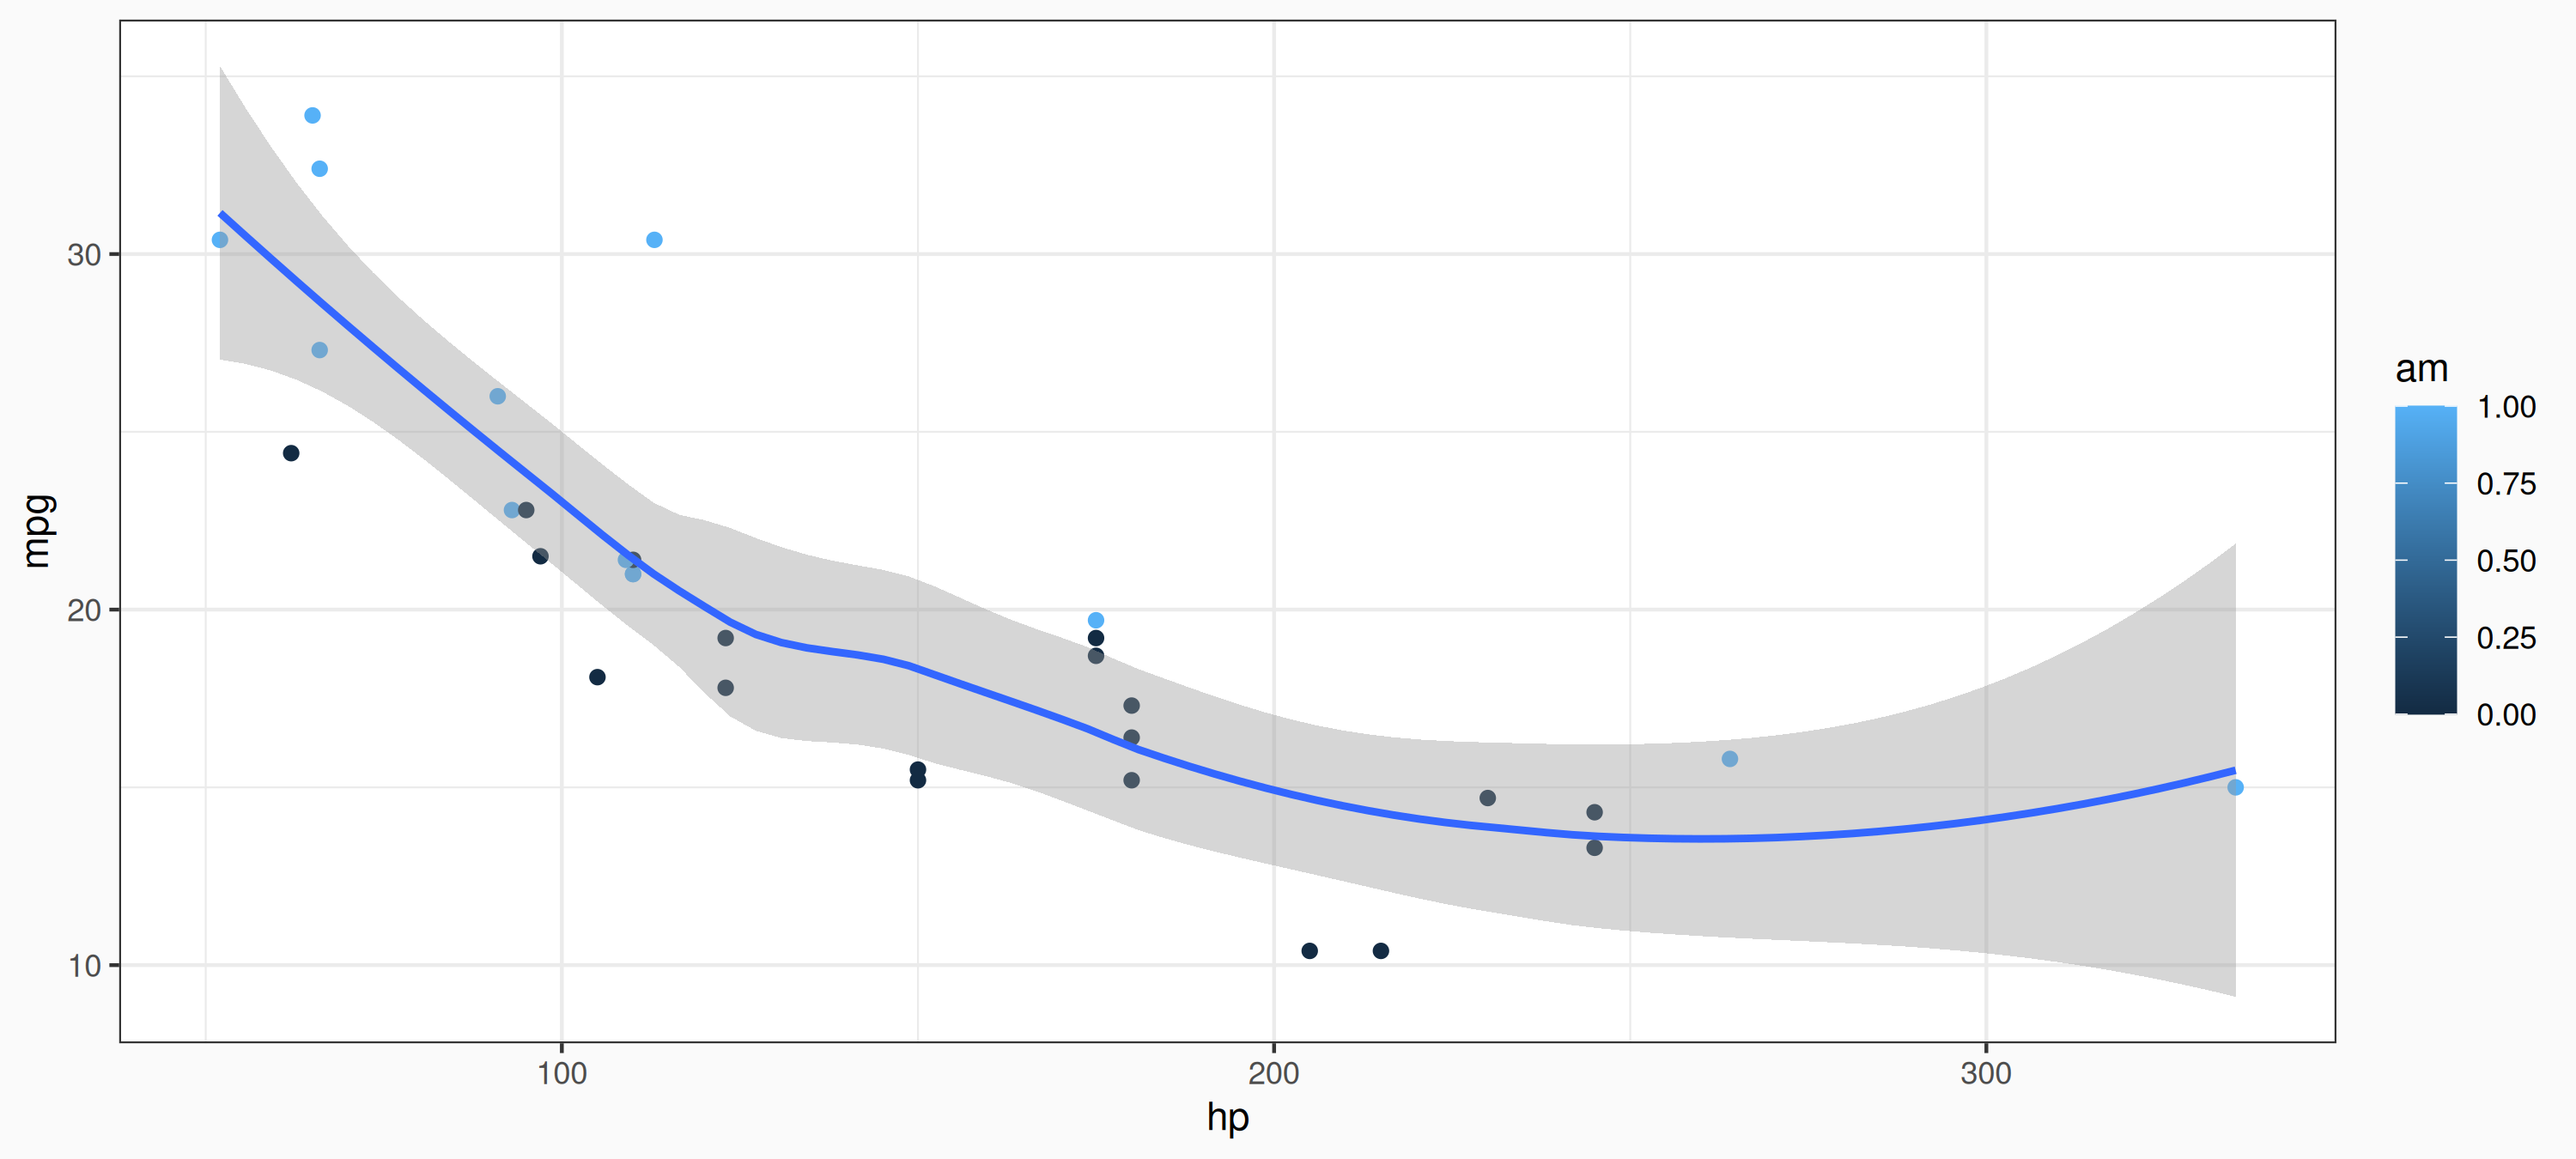
\includegraphics[width=0.55\linewidth,height=\textheight,keepaspectratio]{gb-slides_files/figure-beamer/unnamed-chunk-2-1.png}
\end{center}

Learn more:
\href{https://quarto.org/docs/presentations/revealjs/\#executable-code}{Executable
Code}
\end{frame}

\begin{frame}{A base plot}
\protect\phantomsection\label{a-base-plot}
\begin{tcolorbox}[colback=lightgray!40, colframe=navbargrey, arc=2pt, boxrule=0.5pt, fontupper=\ttfamily\footnotesize]
plot(rnorm(1000),rnorm(1000),xlab="x",ylab="y")
\end{tcolorbox}

\begin{center}
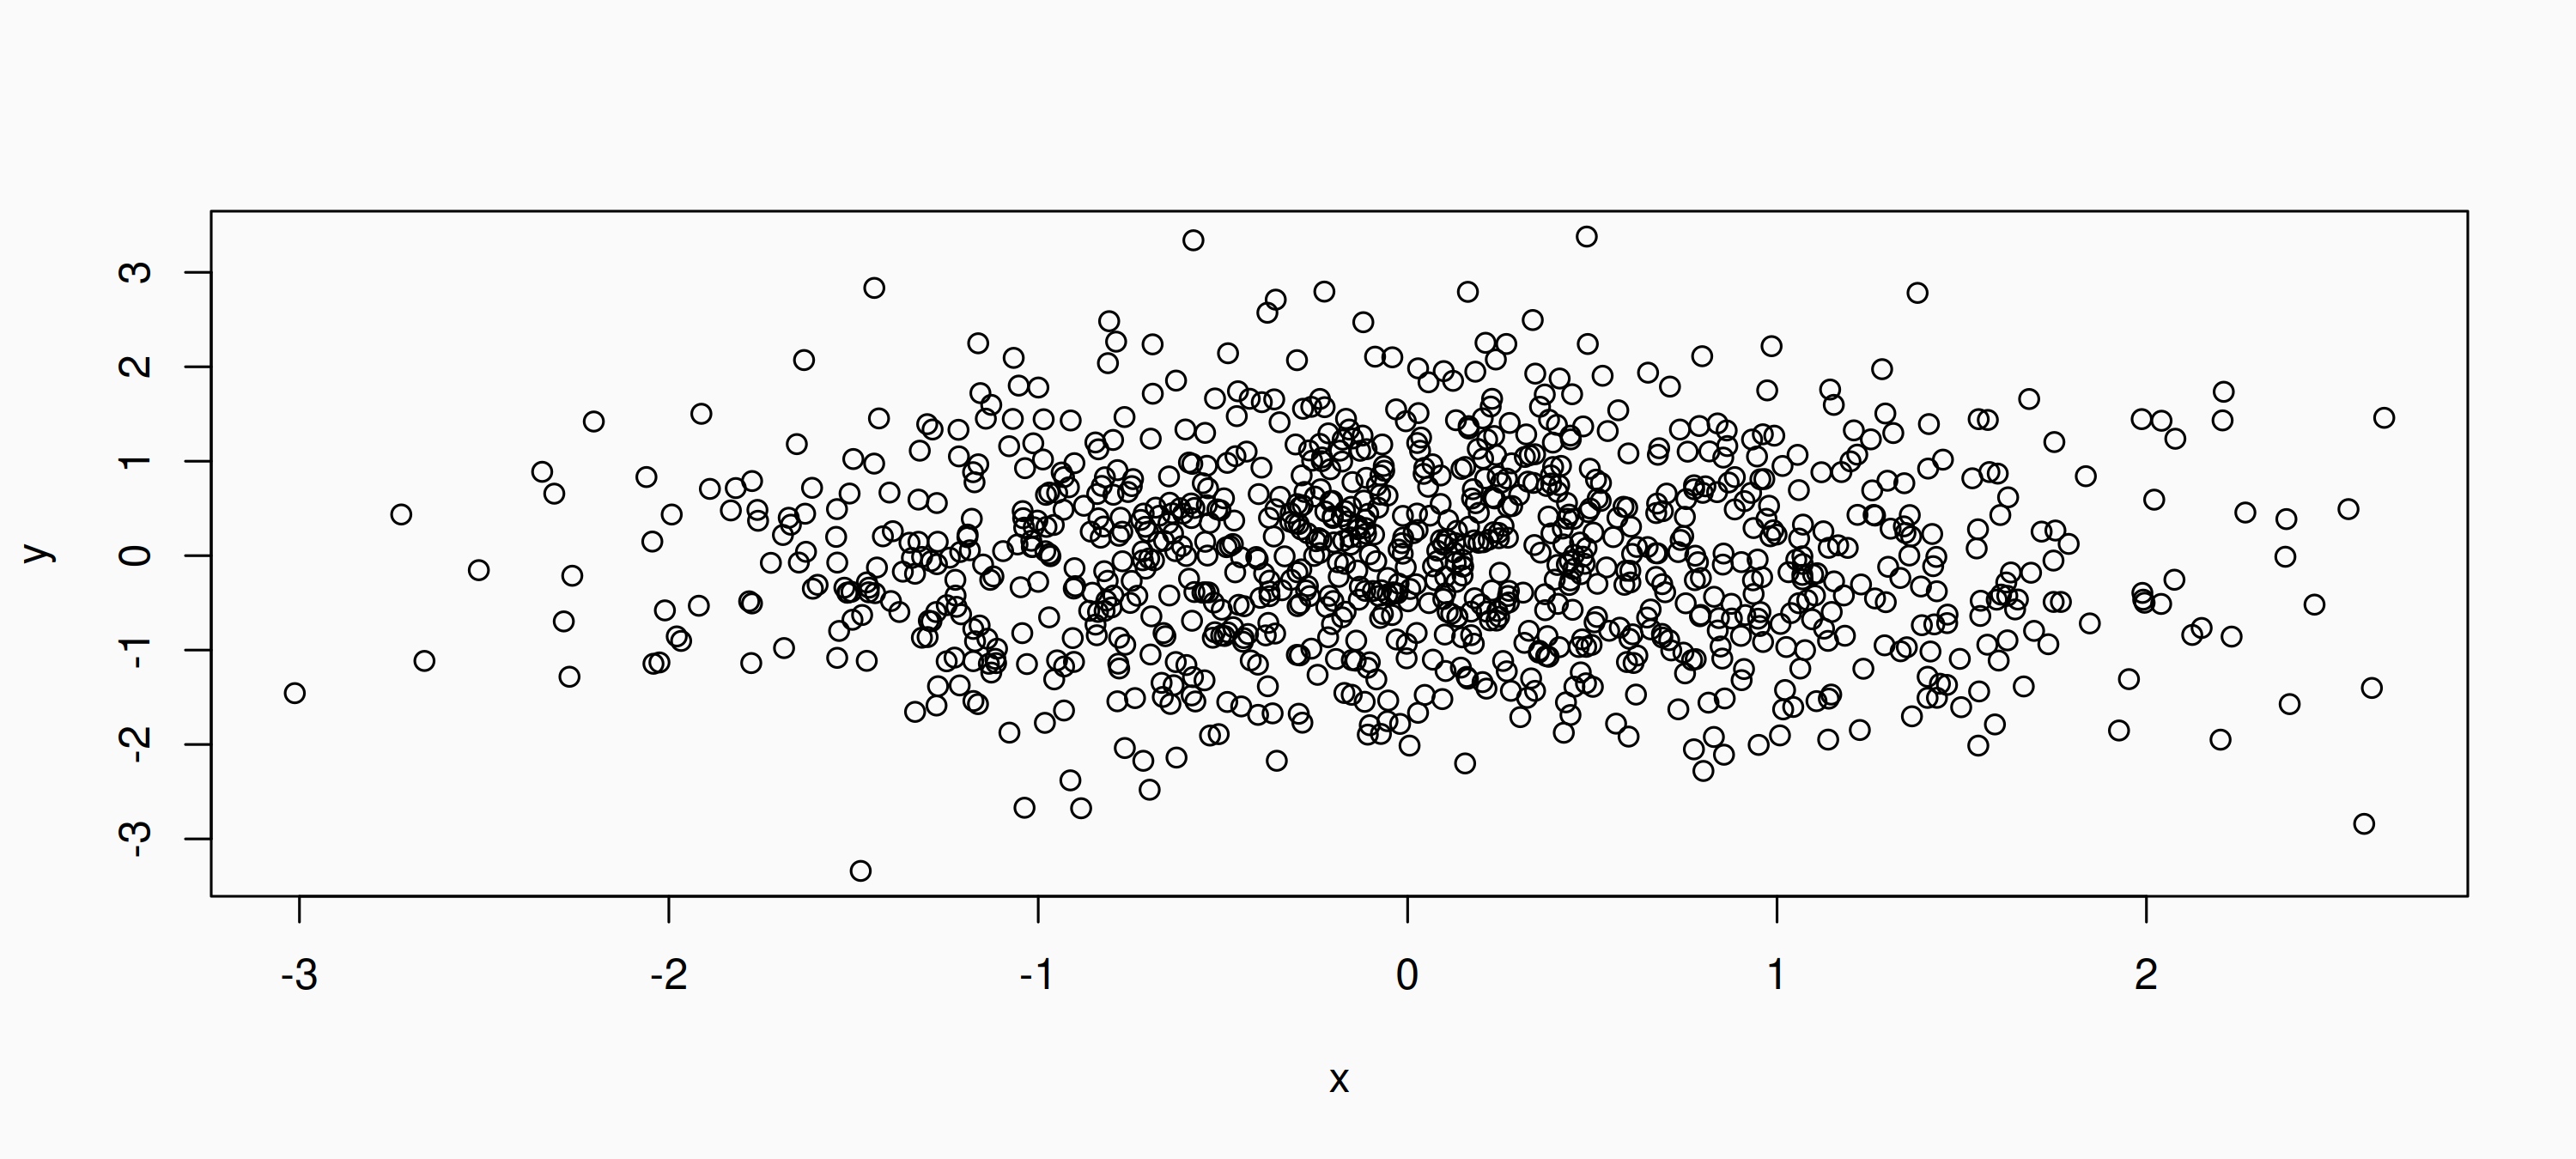
\includegraphics[width=0.55\linewidth,height=\textheight,keepaspectratio]{gb-slides_files/figure-beamer/unnamed-chunk-3-1.png}
\end{center}
\end{frame}

\section{A section}\label{a-section}

\begin{frame}[fragile,noframenumbering]{}
\uclDividerFrameStart{A section}

Using the tag \texttt{\{.divider\}} makes for some nicer \texttt{css}
formatting (especially under \texttt{ucl-revealjs})

\uclDividerFrameEnd
\end{frame}

\begin{frame}{Column Layout}
\protect\phantomsection\label{column-layout}
Arrange content into columns of varying widths:

\begin{columns}[T]
\begin{column}{0.35\linewidth}
\begin{block}{Motor Trend Car Road Tests}
\protect\phantomsection\label{motor-trend-car-road-tests}
The data was extracted from the 1974 Motor Trend US magazine, and
comprises fuel consumption and 10 aspects of automobile design and
performance for 32 automobiles.
\end{block}
\end{column}

\begin{column}{0.03\linewidth}
\end{column}

\begin{column}{0.62\linewidth}
{\def\LTcaptype{none} % do not increment counter
\begin{longtable}[]{@{}lrrrrr@{}}
\toprule\noalign{}
& mpg & cyl & disp & hp & wt \\
\midrule\noalign{}
\endhead
Mazda RX4 & 21.0 & 6 & 160 & 110 & 2.620 \\
Mazda RX4 Wag & 21.0 & 6 & 160 & 110 & 2.875 \\
Datsun 710 & 22.8 & 4 & 108 & 93 & 2.320 \\
Hornet 4 Drive & 21.4 & 6 & 258 & 110 & 3.215 \\
Hornet Sportabout & 18.7 & 8 & 360 & 175 & 3.440 \\
Valiant & 18.1 & 6 & 225 & 105 & 3.460 \\
\bottomrule\noalign{}
\end{longtable}
}
\end{column}
\end{columns}

Learn more:
\href{https://quarto.org/docs/presentations/revealjs/\#multiple-columns}{Multiple
Columns}
\end{frame}

\begin{frame}{Incremental Lists}
\protect\phantomsection\label{incremental-lists}
Lists can optionally be displayed incrementally:

\begin{enumerate}[<+->]
\tightlist
\item
  First item
\item
  Second item
\item
  Third item
\end{enumerate}

\pause

Insert pauses to make other types of content display incrementally.

Learn more:
\href{https://quarto.org/docs/presentations/revealjs/\#incremental-lists}{Incremental
Lists}
\end{frame}

\begin{frame}[fragile]{Fragments}
\protect\phantomsection\label{fragments}
Incremental text display and animation with fragments:

\href{https://quarto.org/docs/presentations/revealjs/advanced.html\#fragment-classes}{Extra
fragment styling / nesting / ordering options}

\uncover<+->{

Fade in

}

\uncover<+->{

Slide up while fading in

}

\uncover<+->{

Slide left while fading in

}

\uncover<+->{

Fade in then semi out

}

\pause

\uncover<+->{

Strike

}

{\color<+->{red}%

Highlight red (but green and blue are also built-in)

}%

\pause

{\color<+->{italian-red}%

Highlight custom colour (defined in \texttt{scss} file or can be added
on the fly)

\begin{tcolorbox}[colback=lightgray!40, colframe=navbargrey, arc=2pt, boxrule=0.5pt, fontupper=\ttfamily\footnotesize]
```{css} \\ \#| echo: false \\ .reveal .slides section .fragment.highlight-itared { \\   opacity: 1; \\   visibility: inherit; \\ } \\ .reveal .slides section .fragment.highlight-itared.visible { \\   color: \#ce2b37; \\ } \\ ``` \\  \\ ::: {.fragment .highlight-itared} \\ Text to highlight here... \\ :::
\end{tcolorbox}

}%

Learn more:
\href{https://quarto.org/docs/presentations/revealjs/advanced.html\#fragments}{Fragments}
\end{frame}

\begin{frame}[fragile]{Fragments (in beamer)}
\protect\phantomsection\label{fragments-in-beamer}
\begin{itemize}
\item
  The file \texttt{beamer-meta.lua} defines a filter to map the code
  \texttt{:::\ \{.fragment\ .highlight-XXX\}}, which is specific to
  \texttt{revealjs}
\item
  More colours can be defined and added to the filter, in the part

  \begin{verbatim}
   local highlight_colors = {
     ["highlight-red"]      = "red",
     ["highlight-green"]    = "green",
     ["highlight-blue"]     = "blue",
     ["highlight-itared"]   = "italian-red",
     ["highlight-itagreen"] = "italian-green",
     ["new-colour"]         = "new-colour"
  }
  \end{verbatim}

  and the \texttt{new-colour} must also be defined in the
  \texttt{ucl-beamer.tex} template (both under
  \texttt{\_extensions/ucl/beamer})
\end{itemize}
\end{frame}




\end{document}
